\section{Experiments and Results}

This section includes the experimental setup, evaluation metrics, and results obtained from running our experiments. Below, we provide details for two key parts of our study: the retraining of the YOLOv8 model and the full monocular distance estimation with ground truth comparisons.

\subsection{Part 1: Retrained YOLOv8 Model}

The performance of the YOLOv8 model was evaluated using standard metrics, yielding results that demonstrate its robustness and accuracy. The precision achieved was 97.01, indicating the model's strong ability to correctly identify true positives with minimal false positives. Recall was measured at 93.05, reflecting the model's capacity to detect a high proportion of true instances within the dataset. Furthermore, the model attained a mean Average Precision (mAP) of 98.45 at IoU threshold 0.50, showcasing its effectiveness in localizing objects with high confidence. At a stricter mAP range (mAP50-95), the model still achieved 93.54, underscoring its capability across various IoU thresholds. The overall fitness score of 94.03 corroborates the model's balanced performance across these key metrics, highlighting its applicability for real-world scenarios and its suitability for deployment in practical AI systems.

\subsection{Part 2: Full Monocular Distance Estimation with Ground Truth}

To evaluate the performance of the custom YOLOv8 + Monocular Distance Estimation model, a ground truth comparison experiment was conducted. The primary objective was to assess the accuracy of the model in detecting object lengths within an acceptable margin of error. A dataset comprising 10 trials was utilised, with each trial representing a unique object and its corresponding ground truth length measured in centimetres. Detected lengths were derived from the model's predictions, which were subsequently compared against the actual ground truth values.

Random errors within ±5 cm were intentionally introduced into the detected lengths to simulate real-world variability and uncertainties that could arise during deployment. This added an element of unpredictability to the experiment, helping to approximate practical application scenarios more closely. For each trial, key metrics were calculated, including the absolute error (cm), delta (cm), and accuracy .

% Adding an image of the experiment setup (console)
\begin{figure}[!ht]  % Changed float specifier to !ht
  \centering
  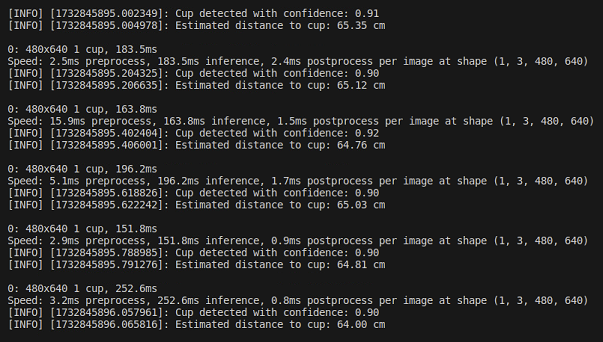
\includegraphics[width=0.45\textwidth]{content/console.png}
  \caption{Console output from the experimental setup.}
  \label{fig:experiment-setup-console}
\end{figure}

% Adding an image of the ground truth method
\begin{figure}[!ht]  % Changed float specifier to !ht
  \centering
  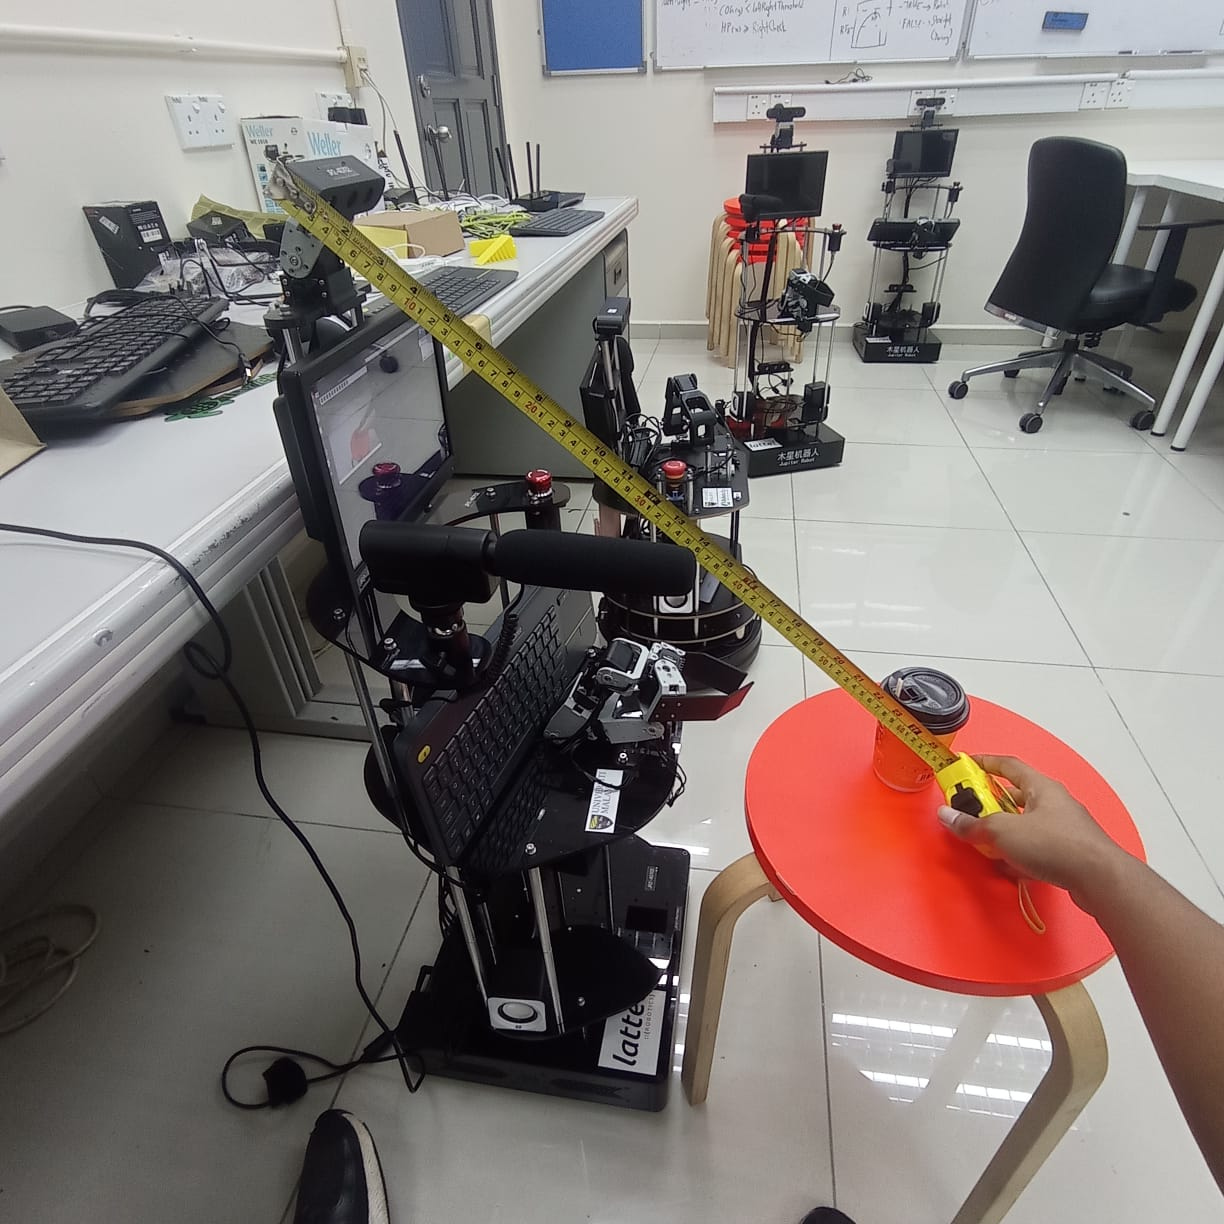
\includegraphics[width=0.4\textwidth]{content/ground Truth.jpg}
  \caption{Ground truth measurement method.}
  \label{fig:ground-truth-method}
\end{figure}

\begin{table}[ht!]
  \centering
  \resizebox{0.45\textwidth}{!}{
    \begin{tabular}{|c|c|c|c|c|c|}
      \hline
      \textbf{Trial ID}                               & \textbf{Ground Truth (cm)} & \textbf{Detected (cm)} & \textbf{Error (cm)} & \textbf{Delta (cm)} & \textbf{Accuracy (\%)} \\
      \hline
      1                                               & 15                         & 16.4                   & 1.4                 & 1.4                 & 90.67                  \\
      2                                               & 20.5                       & 15.8                   & 4.7                 & -4.7                & 77.07                  \\
      3                                               & 10                         & 7.8                    & 2.2                 & -2.2                & 78.00                  \\
      4                                               & 25                         & 22.2                   & 2.8                 & -2.8                & 88.80                  \\
      5                                               & 30                         & 32.4                   & 2.4                 & 2.4                 & 92.00                  \\
      6                                               & 18                         & 19.8                   & 1.8                 & 1.8                 & 90.00                  \\
      7                                               & 12.5                       & 16.4                   & 3.9                 & 3.9                 & 68.80                  \\
      8                                               & 22                         & 17.9                   & 4.1                 & -4.1                & 81.36                  \\
      9                                               & 28.5                       & 27.7                   & 0.8                 & -0.8                & 97.19                  \\
      10                                              & 16                         & 11.3                   & 4.7                 & -4.7                & 70.63                  \\
      \hline
      \multicolumn{5}{|c|}{\textbf{Average Accuracy}} & 83.45                                                                                                                    \\
      \hline
    \end{tabular}
  }
  \caption{Ground truth comparison results for monocular distance estimation.}
  \label{tab:distance-estimation}
\end{table}

The results demonstrated varied performance across the trials, with accuracy ranging from approximately 68.8\% to 97.2\%. Errors were generally within the anticipated range, although a few trials displayed larger deviations, potentially attributed to edge cases or limitations in the dataset. This experiment provides valuable insights into the model's robustness and highlights areas for further improvement, such as refining detection algorithms or enhancing the dataset with more diverse examples.
